\documentclass[10pt,a4paper,oneside]{book}

\begin{document}

\chapter{Laboratory Instructions}

This laboratory is divided into two different experiments. In the first part, you will perform STORM imaging of cells. One type of organelle in the cell (for example, the microtubules) has been labeled with fluorescent markers. You will image these markers and reconstruct the microtubule network in the cell. In the second part, you will image DNA origami nanorulers as part of a metrology experiment. The goal is to asses the precision of the microscope and the SMLM technique.

\section{Safety}

\fbox{
    \parbox{\textwidth}{\textbf{WARNING} The buffers used in SMLM contain highly toxic chemicals. Always follow proper laboratory safety procedures and wear the proper personal protective equipment. Please alert a teaching assistant immediately if any of the buffer touches you.}
}\newline

\noindent\fbox{
    \parbox{\textwidth}{\textbf{WARNING} SMLM imaging requires the use of high-powered lasers. A safety interlock over the objective is in place to avoid accidental exposure. Do not attempt to bypass the interlock.}
}\newline

\section{Common Procedures}

The following procedures are common to both experiments.

\subsection{Description of the Microscope}

The microscope is an Abbelight SAFe 180. It consists of an Olympus IX83 microscope, an Abbelight scanning illumination system, an Oxxius laser engine, a Hamamatsu ORCA-Fusion digital CMOS camera, and other components. Some of these components are labeled in \autoref{fig:microscope} and \autoref{fig:electronics}.

\begin{figure}[ht]
    \centering
    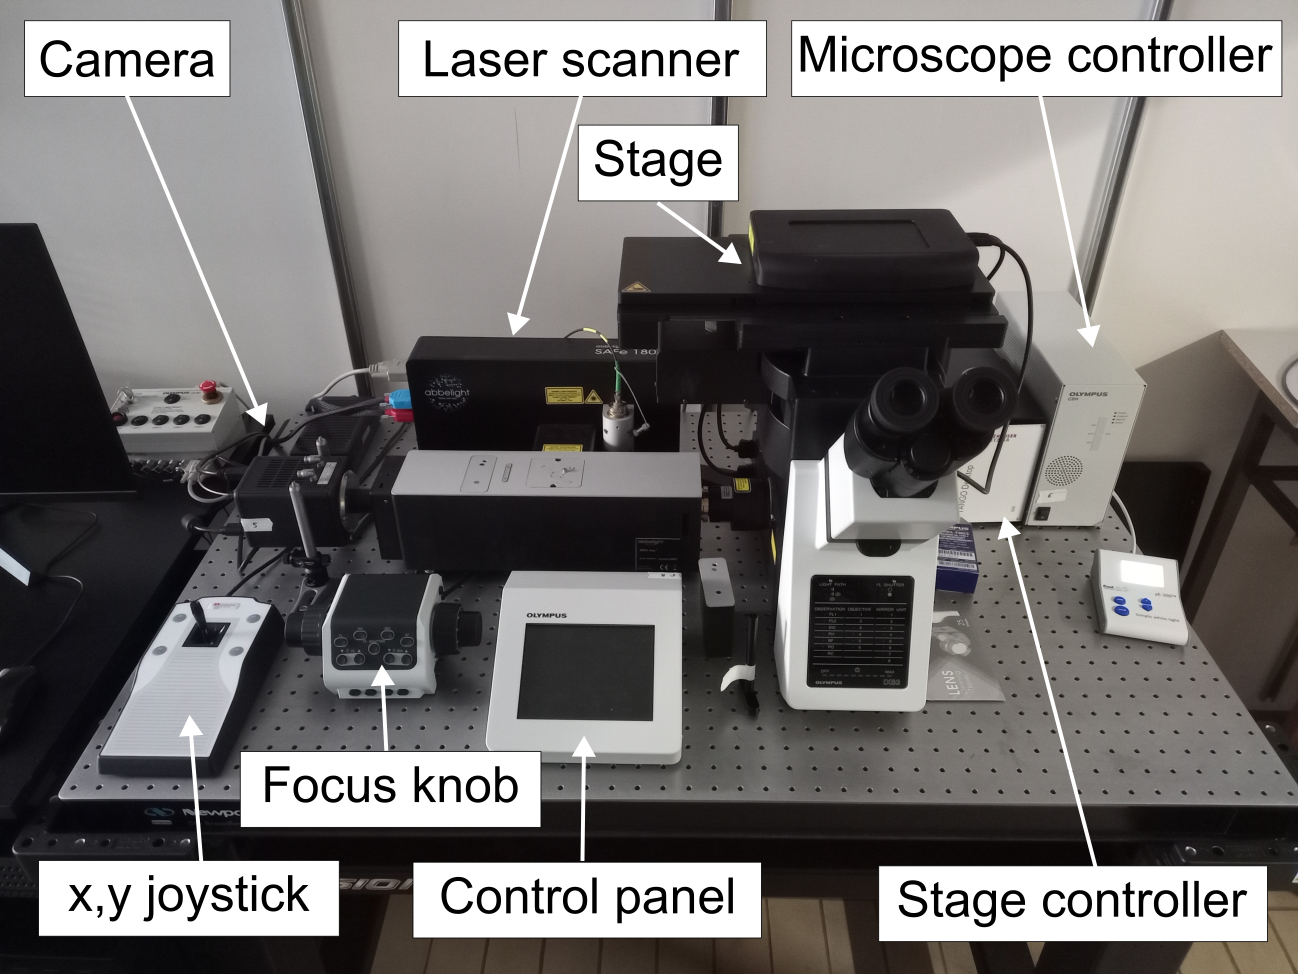
\includegraphics[width=0.75\textwidth]{microscope.png}
    \caption{The primary components of the microscope used in this course.}
    \label{fig:microscope}
\end{figure}

\begin{figure}[ht]
    \centering
    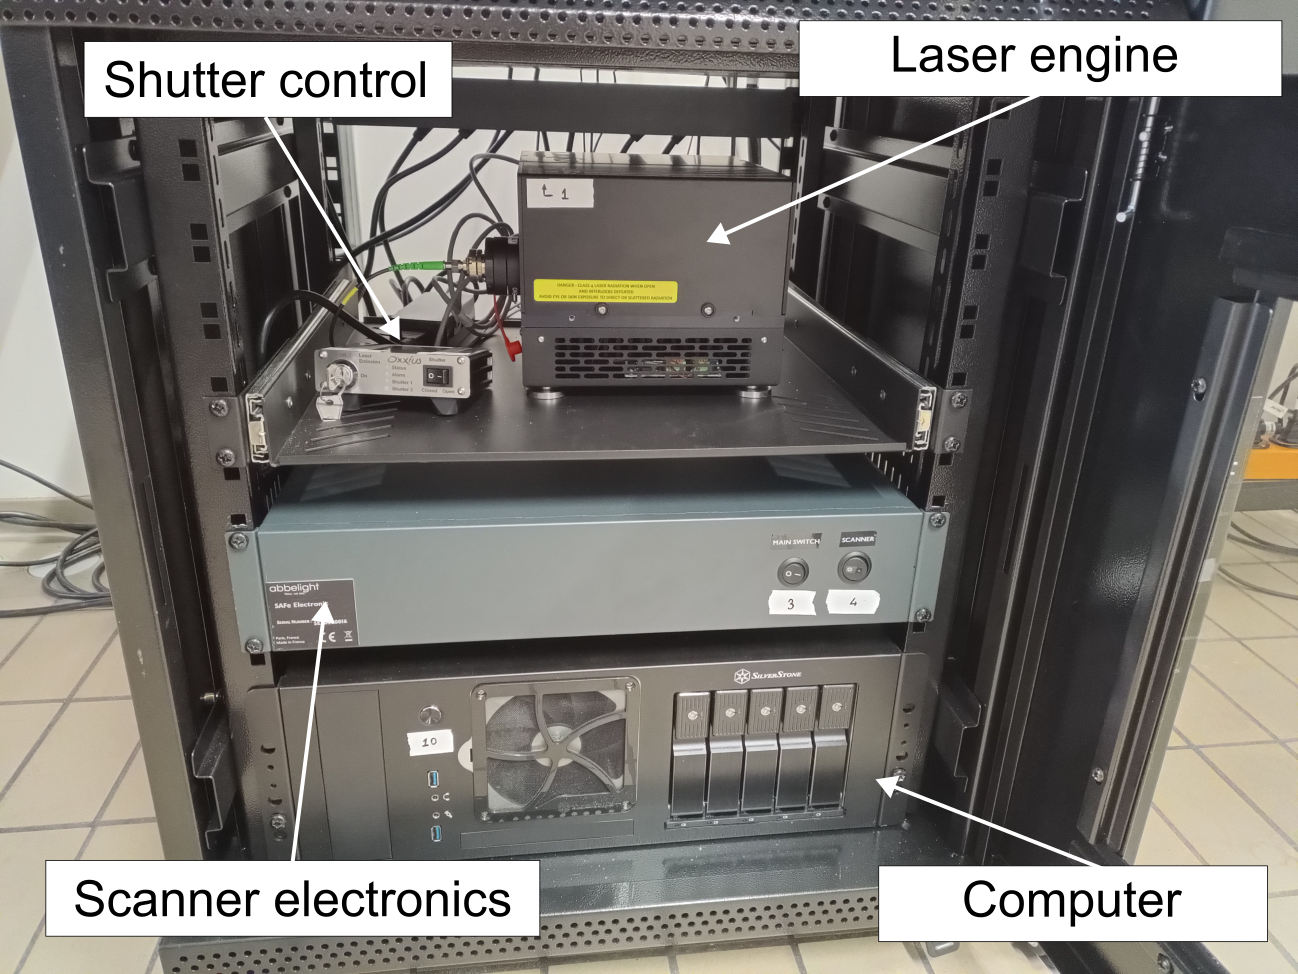
\includegraphics[width=0.75\textwidth]{electronics.png}
    \caption{Electronics and laser source for the microscope.}
    \label{fig:electronics}
\end{figure}

You may learn more about the microscope here: \url{https://www.abbelight.com/solutions/bioimaging-instruments/}.

\subsection{Turn On the Microscope}\label{sec:startup}

To turn on the microscope, turn on the following components in this order. There should be pieces of tape with numbers on them and attached to the actual devices to aid you.

\begin{enumerate}
    \item Laser engine
    \item Laser safety key on the shutter controller
    \item Scanner electronics: main switch
    \item Scanner electronics: scanner
    \item Camera \newline Wait for the status light to turn green before proceeding.
    \item Olympus CBH microscope controller
    \item Maerhaeuser Tango Desktop stage controller
    \item Olympus control panel \newline Wait for the "Start Operation" button to appear, then press it to continue. This can take about one minute.
    \item Laser shutter
    \item The computer
\end{enumerate}

\subsection{Mount the Sample}\label{sec:mount-sample}

The sample is mounted in two steps: 1. mount the sample coverslip onto a glass cavity well slide, and 2. mount the slide/coverslip combination onto the microscope.

\subsubsection{Mount the Coverslip onto the Slide}

\fbox{
    \parbox{\textwidth}{\textbf{WARNING} Gloves and eye protection must be worn for this procedure.}
}\newline

A video tutorial describing this process may be found at \url{https://drive.google.com/file/d/1czRAzCVn1dEPEgESOuVnm_-1_1xvhQnW/view?usp=sharing}. You need to be signed in with your EPFL account to view the video.

Mounting the coverslip onto the slide requires the following materials:

\begin{itemize}
    \item{Glass cavity well slide}
    \item{Coverslip with sample}
    \item{Buffer kit}
    \item{Picodent sealant (both yellow and blue components)}
    \item{Tweezers}
    \item{Pipettes}
    \item{200 $\mu$L and 1 mL pipette tips}
    \item{Paper towels}
\end{itemize}

Begin by mixing the components of the buffer kit. Add 10 $\mu$L of solution from the green tube the blue tube. \textbf{Be sure to never exceed the soft stop on the pipette because you may accidentally suck solution into it.} Mix the solution by pipetting it up and down several times. Next, add 6 $\mu$L of solution from the red tube to blue tube. Mix the solution again. The buffer is now ready to use.

For the next step, load 175 $\mu$L of the prepared buffer solution into the cavity slide using a 1 mL pipette tip. Then, using tweezers, gently pick up the coverslip with the cell sample on it and place it over the cavity well with the sample side facing into the buffer. Gently remove any excess buffer by placing a paper towel over the slide.

If there is a bubble, \textbf{very gently} slide the coverslip to the side until the bubble is exposed. Add a tiny bit more buffer, then slide the coverslip back to the center of the well. Remove any excess buffer as before.

Finally, mix together equal amounts of the Picodent sealant's yellow and blue components in a small dish with a 1 mL pipette tip. When properly mixed, the sealant will turn to a light green color. Using the same tip, add the sealant around the entirety of the coverslip edge to prevent any buffer from leaking out.

\subsubsection{Mount the Slide onto the Microscope}

\autoref{fig:objective-sample} illustrates how the sample should be mounted onto the microscope. The side with the sample must face in towards the buffer, and the side of the slide with the coverslip must be closest to the microscope objective.

\begin{figure}[ht]
    \centering
    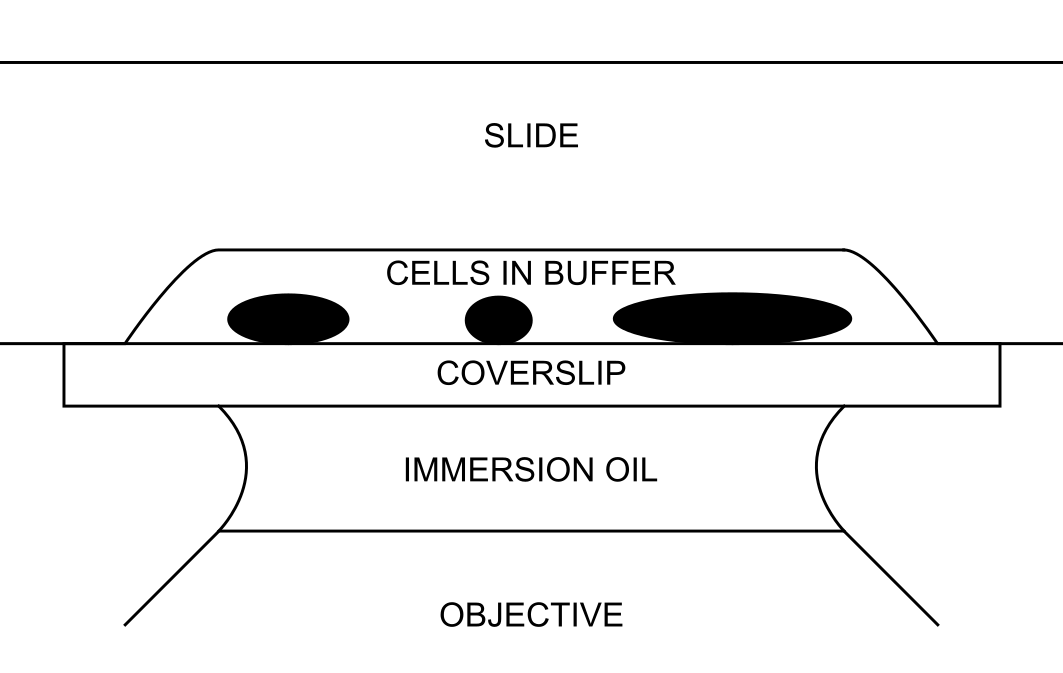
\includegraphics[width=0.75\textwidth]{oil-immersion-objective-with-sample.png}
    \caption{Illustration of the sample/objective space showing the relative positions of the various components and media. This illustration is not to scale!}
    \label{fig:objective-sample}
\end{figure}

Mounting the slide requires only immersion oil.

To mount the slide onto the microscope, first remove the black safety cover over the objective. Place a small drop of immersion oil on top of the objective lens. Only one small drop is necessary! The immersion oil allows light rays at large angles to the microscope axis to enter the objective's aperture. This increases the resolution of the microscope.

Next, turn the focus knob so that the microscope objective is all the way down as indicated by the yellow line in the objective position indicator section of the microscope control panel. Then, place the slide into the sliding black metallic mounts and gently push them together until the slide is secure. Ensure that the coverslip is centered over the objective. Finally, turn the focus knob to raise the objective slowly until it is just touching the oil. You will know when the objective is touching the oil because you can see the oil spreading out underneath the objective. A video that illustrates this effect may be found at \url{https://drive.google.com/file/d/1IC5Azq-raW6_jVSnuBDrSsZ0OsQYxoPK/view?usp=sharing}.

\subsection{Turn Off the Microscope}

Turn off the components in the opposite order as in \autoref{sec:startup}.

\subsection{Remove Oil From the Objective}\label{sec:remove-oil}

\subsubsection{Materials}

\begin{itemize}
    \item{Ethanol}
    \item{Lens cleaning tissue}
    \item{Tweezers}
\end{itemize}

The oil must be removed from the objective after imaging, and sometimes during imaging if there is dust in the oil. To do this, use lens cleaning solution and lens tissue to clean the objective. The lens tissue should be folded into a small square and wetted with the cleaning solution. In this laboratory, ethanol is used as the solution, though this can vary with objective manufacturers. Avoid touching the area of the tissue that you will use to clean the objective. After wetting, gently wipe the objective with the lens tissue, slowly moving the tissue across the objective in one direction. Repeat the process if oil remains.

A video demonstration on cleaning objectives may be found at \url{https://www.youtube.com/watch?v=Tz4Dy5D6kdw}.

\section{Experiment 1 - STORM Imaging of Cells}

\subsection{Materials}

\begin{itemize}
    \item{Mounted cell sample (see \ref{sec:mount-sample})}
    \item{Lens cleaning products (see \ref{sec:remove-oil})}
\end{itemize}

\subsection{Procedure}

\subsubsection{Setup the Microscope Configuration}

After mounting the sample and making contact with the immersion oil (\ref{sec:mount-sample}), you should start the imaging software which is called \textbf{NEO Live Imaging}. You will see a screen like the one in \autoref{fig:liveimaging-startup}.

\begin{figure}[ht]
    \centering
    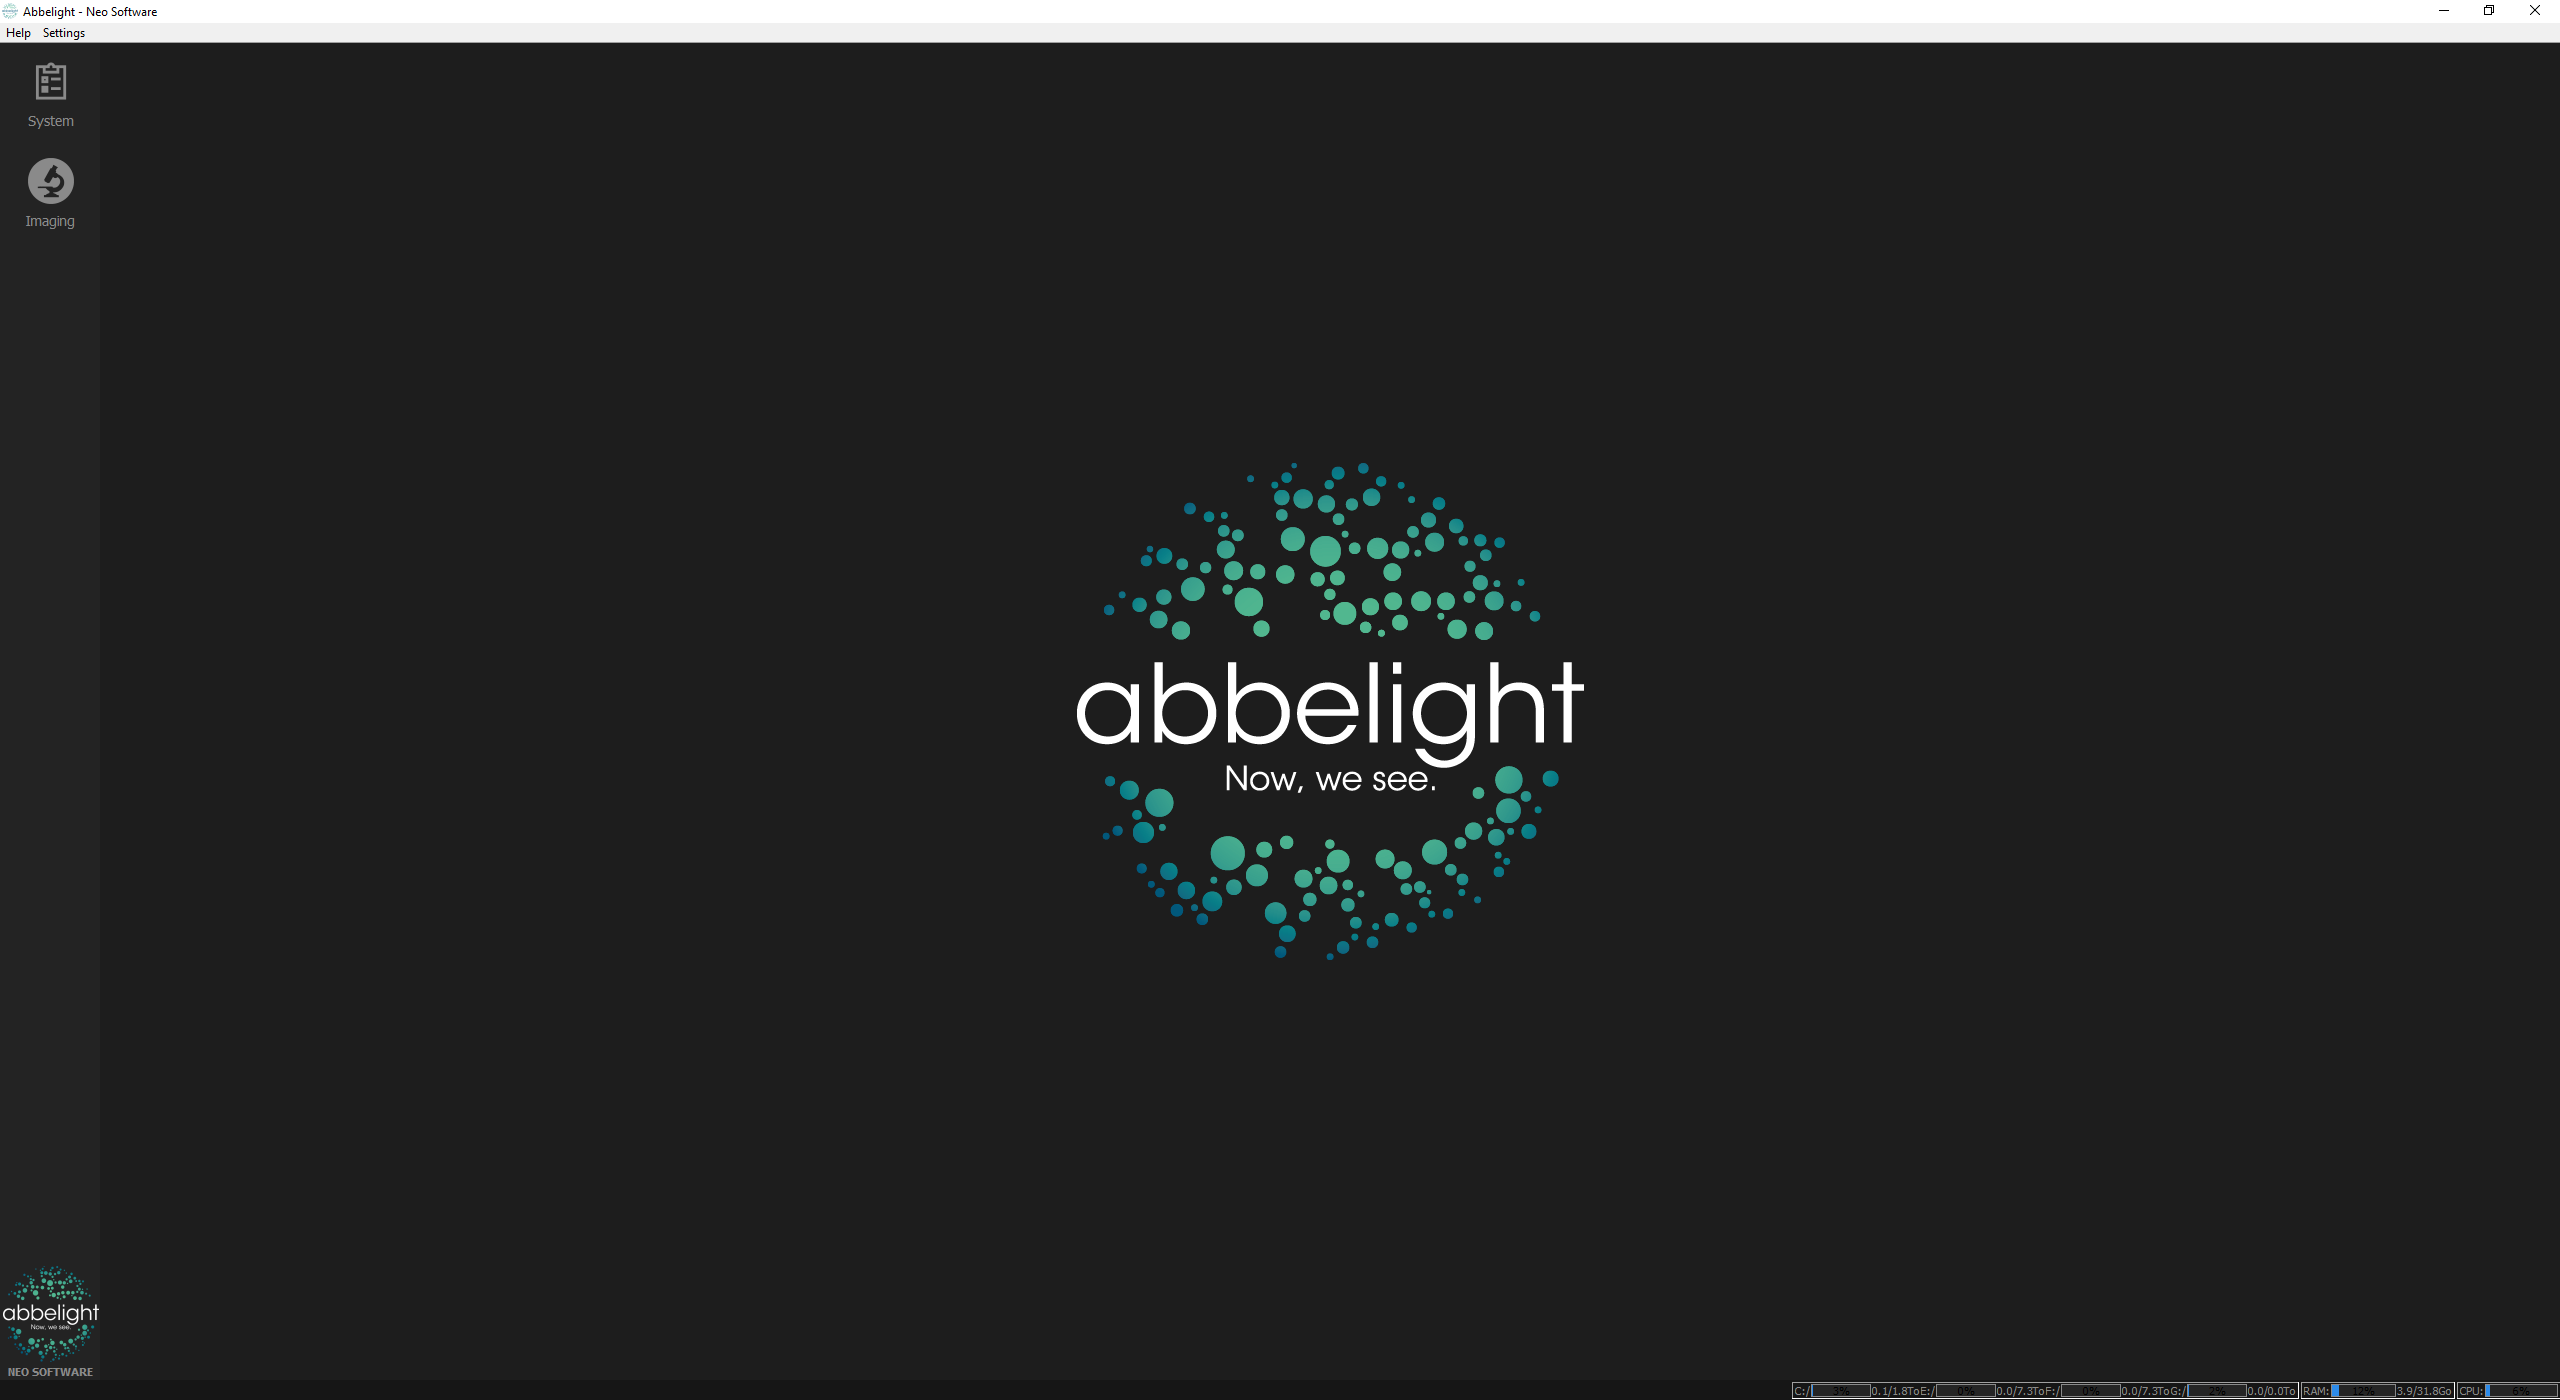
\includegraphics[width=0.75\textwidth]{liveimaging-startup.png}
    \caption{The NEO Live Imaging screen immediately after startup.}
    \label{fig:liveimaging-startup}
\end{figure}

From this screen, you can access two different modes of the software. The first is the `System' mode, which allows you to configure the microscope for different imaging modalities. The second mode is called `Imaging'. While in imaging mode, you directly control the invididual components of the microscope to acquire images.

Click `System'. You will see a screen like the one in \autoref{fig:liveimaging-system}. Clicking on `Hardware Configuration' will reveal a screen like \autoref{fig:liveimaging-hardware-config}. Ensure that the microscope is correct. It should be the `SAFe 180'. Also ensure that the resolution is set to `Nanoscopy' and that `2D' is selected. (3D imaging requires the insertion of an additional lens and a calibration step.) Finally, you can see the pixel size on the sample, which is the camera's physical pixel size divided by the magnification of the microscope. For a 100x objective, the pixel size should be about 108 nm.

\begin{figure}[ht]
    \centering
    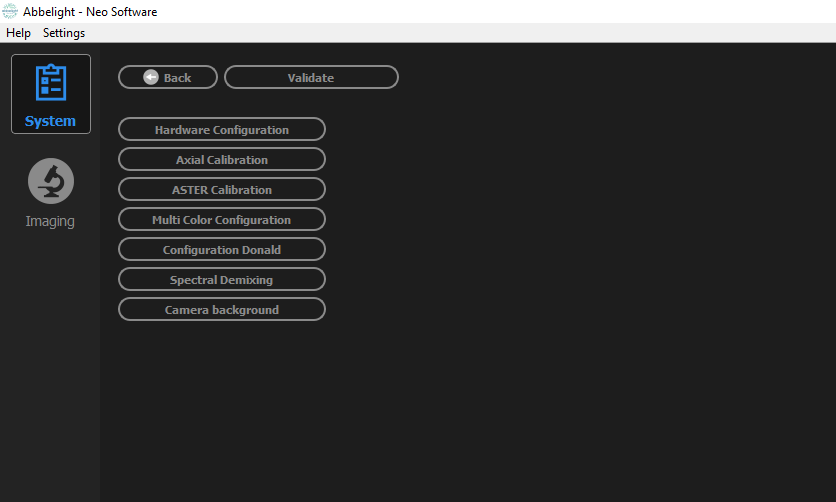
\includegraphics[width=1.0\textwidth]{liveimaging-system.png}
    \caption{The NEO Live Imaging screen in `System' mode.}
    \label{fig:liveimaging-system}
\end{figure}

\begin{figure}[ht]
    \centering
    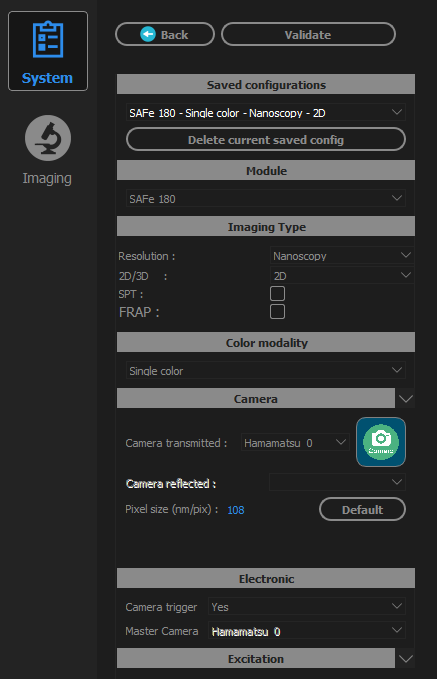
\includegraphics[height=0.5\textheight]{liveimaging-hardware-config.png}
    \caption{The NEO Live Imaging screen showing the current hardware configuration.}
    \label{fig:liveimaging-hardware-config}
\end{figure}

From this screen, you can also select the `Show Optical Path' button to see an illustration of the excitation and emission light paths through the microscope.

If everything looks good, click the `Back' button to go back to the `System' screen.

\subsubsection{Find the Sample}

\fbox{
    \parbox{\textwidth}{\textbf{TIP} It can help to turn off the room lights and close the window shades to reduce the amount of ambient light hitting the camera.}
}\newline

Now you will try to find the sample in the focal plane of the microscope. To start, click the `Imaging' button to put the microscope into imaging mode. Next, start a live stream from the camera by clicking the play button with the label `Start Preview'. You should now see a live image from the camera. The live stream will contain only noise.

Ensure that the metallic safety cover is in place over the objective and sample. If it is not, the lasers will not turn on. Turn on the red 642 nm laser by first selecting the `Settings' button to enable the laser controls. Then, toggle the radio button next to the \textbf{red} slider. Slide the slider a small amount to the right to increase the power slightly.

With the laser on, adjust the focus slowly to try and find the sample. You may need to increase the laser power a small amount and/or move the sample stage with the joystick. When the sample is in focus, you should see a clear image of the cells. Out-of-focus images will appear blurry, as in \autoref{fig:in-vs-out-of-focus}. If, after several minutes, you are unable to find the sample, ask for help. It could be that the cells have detached from the coverslip, in which case you would need to mount a new sample.

\begin{figure}[ht]
    \centering
    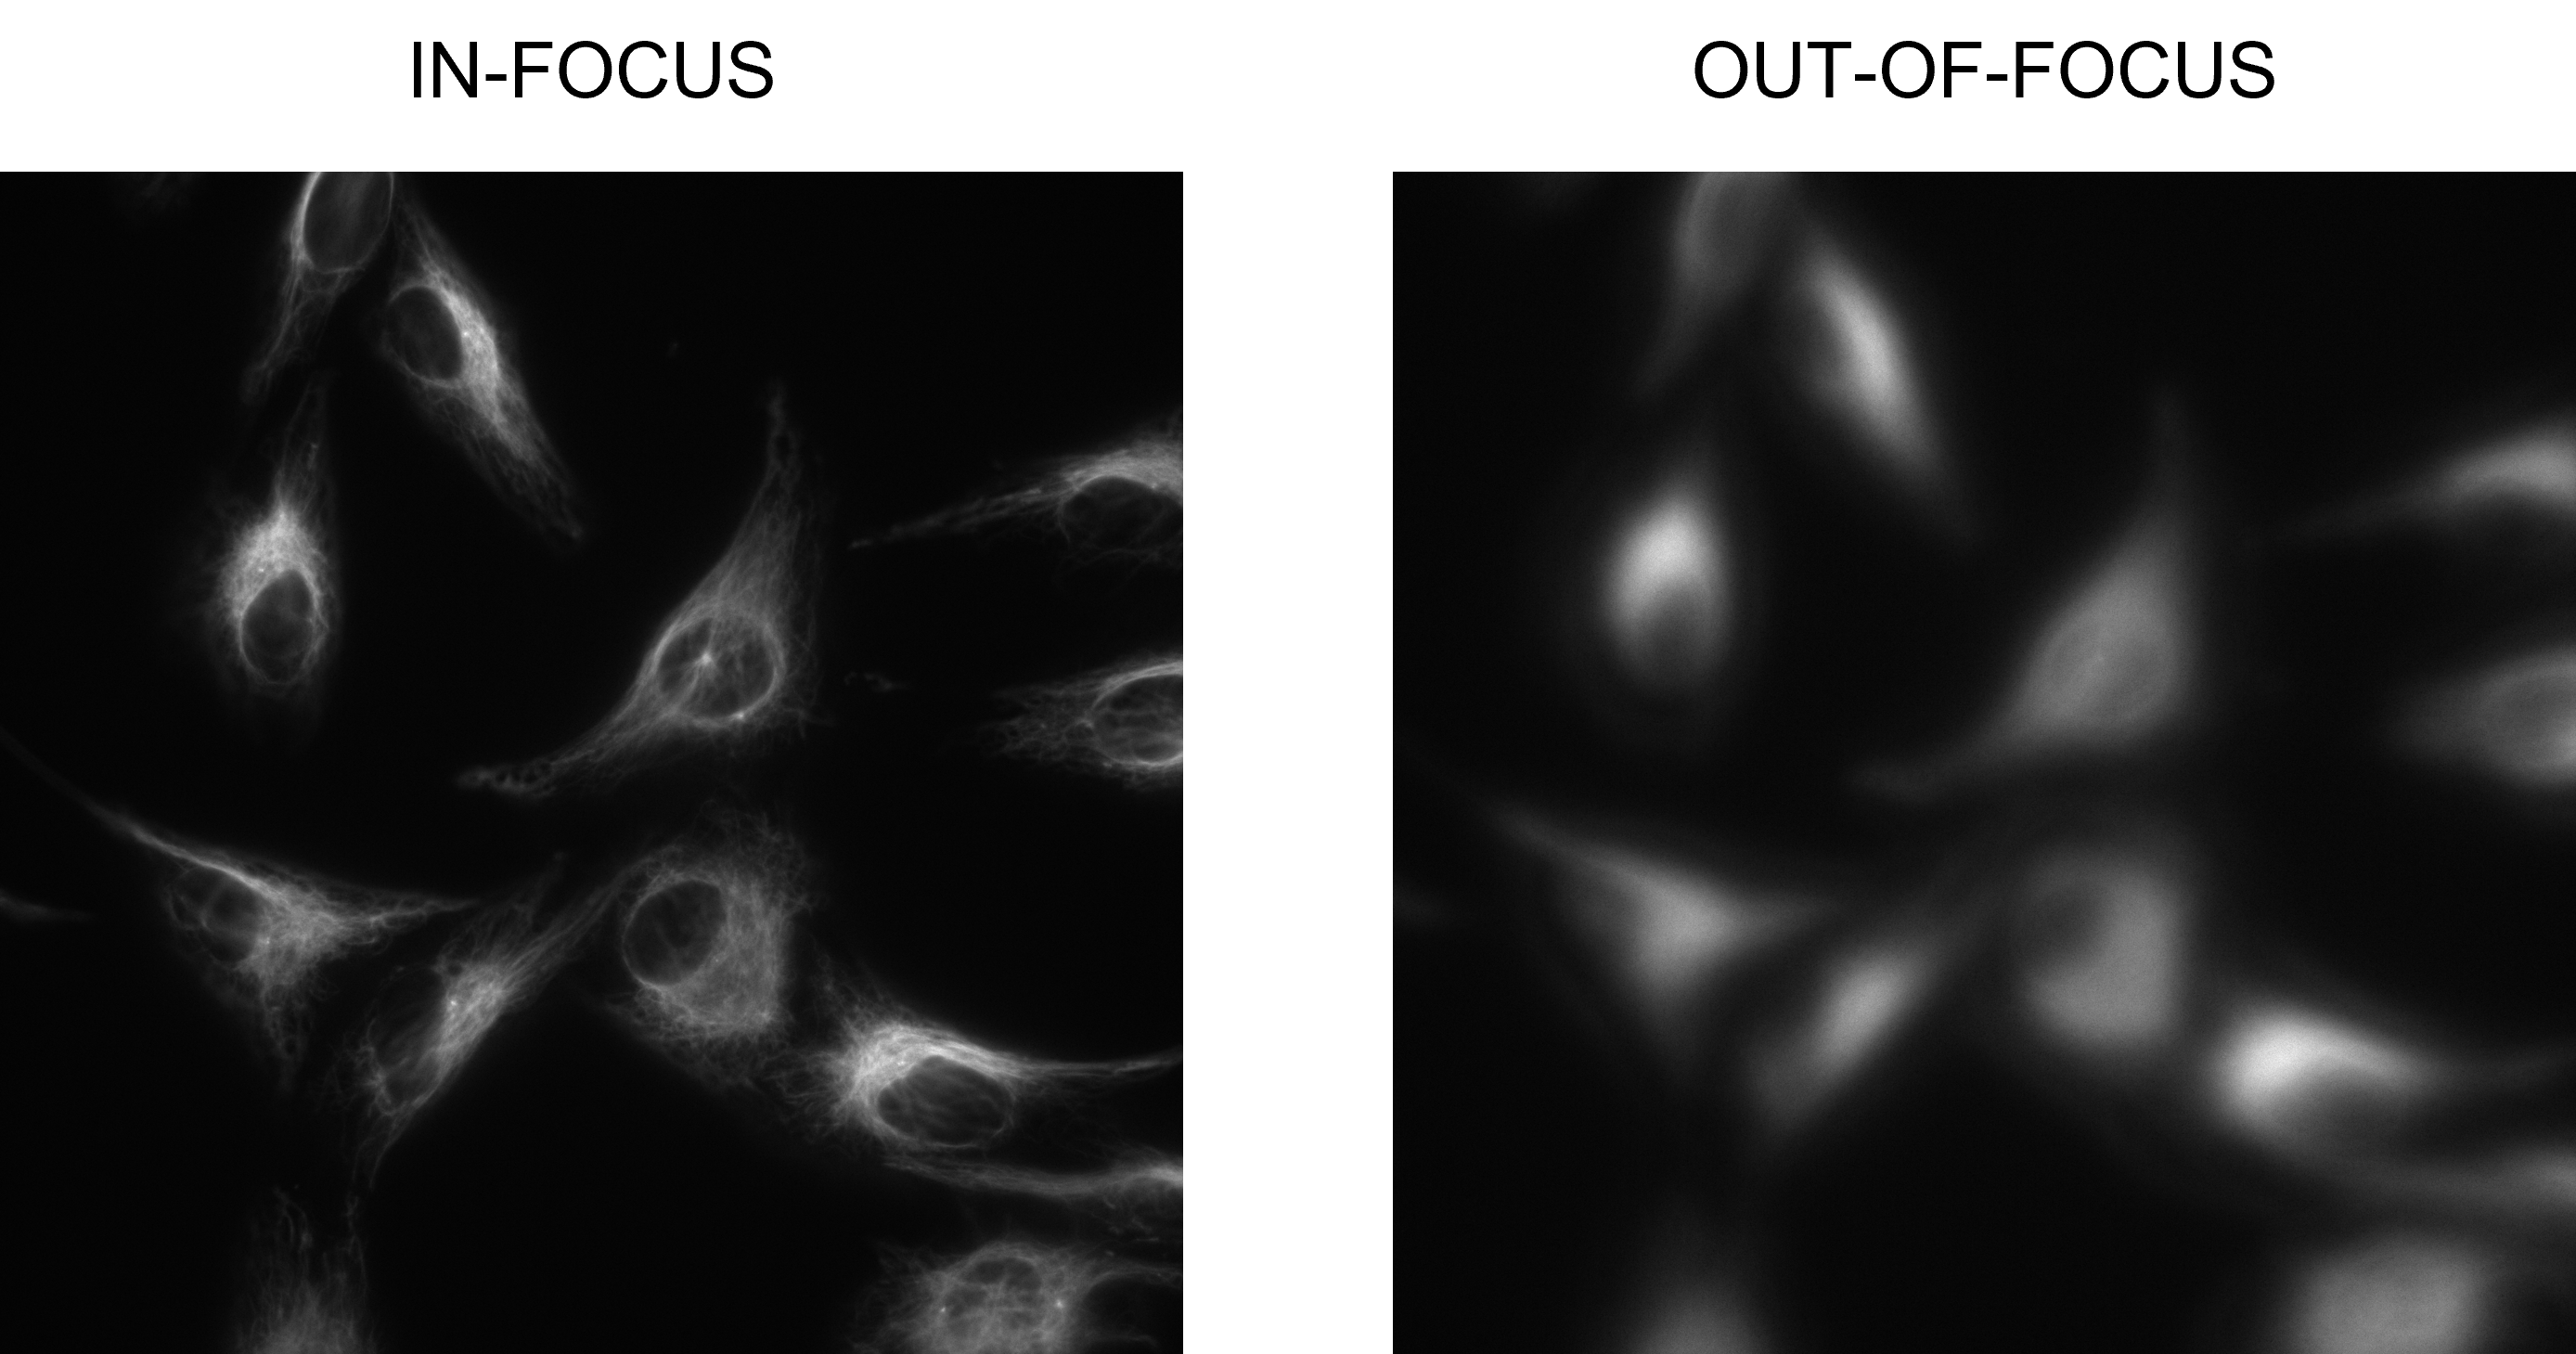
\includegraphics[width=1.0\textwidth]{in-vs-out-of-focus.png}
    \caption{An in-focus image of microtubules in COS7 cells (left) and an out-of-focus image (right). Images courtesy of Matt Lycas.}
    \label{fig:in-vs-out-of-focus}
\end{figure}

\subsubsection{Setup a STORM Acquisition}

A STORM acquisiton is a series of frames recorded from the sample in which the fluorophores are blinking on and off. To setup a new acquisition, first create a project by clicking the `New Project' button. You will be prompted to enter a name for the project, as well as a path to the project data. The path should be \textbf{Documents/acquisition/YYYY-MM-DD-NAME1-NAME2} where `YYYY-MM-DD' are the year, month, and day of the acquisition. `NAME1' and `NAME2' are you and your partner's last names. Once finished, click `OK'. You will see the project appear in the project explorer pane. For the moment, there are no files in the project.

Next, start a live preview. Increase the red laser power until the fluorescent molecules start to blink on and off rapidly. Try to set the power so that there are no overlapping images of individual fluorescent molecules in any one frame. In the `Settings' window, adjust the exposure time and the number of frames. Common values are 50 ms exporsures and 10,000 frames. Also ensure that `EPI' (epi-illumination) is selected for the illumination mode. The settings will look similar to those in \autoref{fig:liveimaging-imaging-settings}.

\begin{figure}[ht]
    \centering
    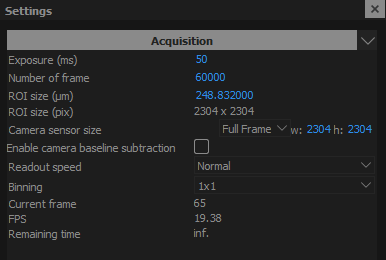
\includegraphics[width=0.75\textwidth]{liveimaging-imaging-settings.png}
    \caption{The NEO Live Imaging screen showing the default acquisition settings. Note the exposure time and the number of frames.}
    \label{fig:liveimaging-imaging-settings}
\end{figure}

For the next step, double click in the window containing the live stream. This will create a green box to define a region of interest, or ROI. The area inside the ROI will be acquired during the acquisition.

\fbox{
    \parbox{\textwidth}{\textbf{TIP} Always use a ROI. Using the full camera frame will create very large datasets that are difficult to work with.}
}\newline

Good ROI sizes are between $25 \, \mu m\times 25 \, \mu m$ and $100 \, \mu m\times 100 \, \mu m$, which is large enough to cover about one cell.

At this point, everything is set. Click the `Start' button to begin the acquisition. At 50 ms and 10,000 frames, an acquisiton will take about 8 minutes. You can see how many frames have been acquired in the settings pane. When the acquisition is finished, you will see new files appear in the project explorer pane for this acquisition.

\section{Experiment 2 - Nanoscale Optical Metrology with SMLM}


\end{document}
